\chapter[Proposta]{Formulação do Problema e Métodos}
\label{proposta}

Este capítulo descreve a proposta computacional avaliada nesta monografia. O foco é formalizar o TSP-SD-ATP, apresentar a estrutura de implementação e detalhar como GA, PSO, ACO, busca exaustiva e lower bound foram integrados ao mesmo pipeline experimental. Conforme a orientação do template institucional, a revisão bibliográfica fica concentrada no Capítulo~\ref{fundamentacao}; aqui são descritas as escolhas efetivamente implementadas.

\section{Formulação do Problema}

Uma instância é definida por um conjunto de pontos bidimensionais $V=\{0,1,\ldots,n-1\}$. O nó $0$ é a base de partida e retorno do drone. Os demais nós, $V'=V\setminus\{0\}$, são pontos de interesse que devem ser visitados exatamente uma vez. Uma rota factível é uma permutação $\pi$ dos nós de $V'$.

O diferencial do TSP-SD-ATP está na avaliação da rota. Em vez de uma matriz $D[j][k]$, a implementação usa um tensor 3D $G[anterior][atual][proximo]$. Cada entrada armazena o custo de seguir de `atual' para `proximo' considerando que o nó visitado imediatamente antes foi `anterior'. O custo soma distância euclidiana e penalidade angular normalizada, conforme a Equação~\ref{eq:custo}.

\begin{figure}[htbp]
  \centering
  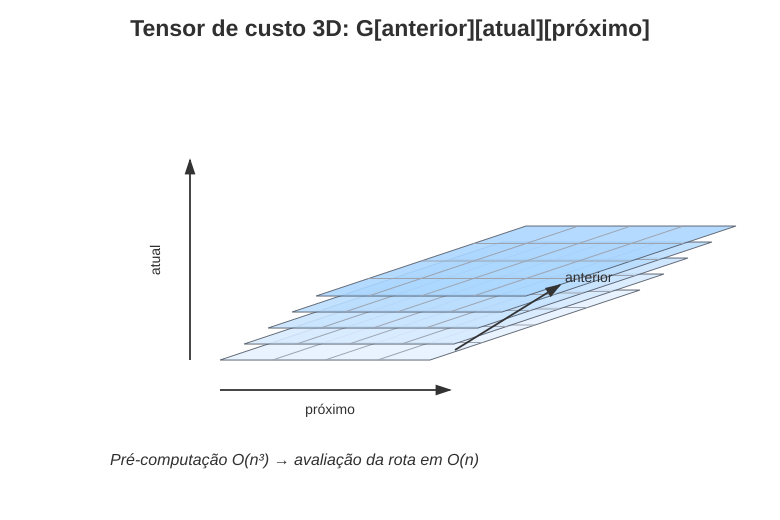
\includegraphics[width=0.76\textwidth]{figs/diagram-tensor-3d.png}
  \caption{Representação do tensor 3D de custos usado para avaliar transições dependentes da sequência. Fonte: elaborado pelo autor.}
  \label{fig:tensor-3d}
\end{figure}

A função objetivo percorre a permutação de pontos de interesse, soma a partida da base, as transições internas e o retorno à base. Após a pré-computação do tensor, uma rota é avaliada em $O(n)$, pois cada passo consulta diretamente uma entrada de $G$. A pré-computação exige $O(n^3)$ entradas, custo aceitável para as instâncias estudadas.

\section{Arquitetura da Implementação}

A implementação foi desenvolvida em Go e organizada em pacotes. O pacote `points' representa os pontos bidimensionais e a geração de instâncias. O pacote `graph' cria o tensor de custos e calcula o \textit{makespan}. O pacote `optimization' contém os métodos de otimização. O pacote `cmd' expõe a interface de linha de comando baseada em Cobra, e `shared/reporting' registra os resultados estruturados.

O fluxo experimental parte de arquivos `.points', gera ou carrega arquivos `.graph' e executa um comando de otimização. Cada execução produz três artefatos: um resumo final (`summary'), um histórico de melhorias (`evolution') e uma decomposição temporal (`timing'). O identificador da execução combina instância, método, semente e hash dos parâmetros, reduzindo o risco de sobrescrever resultados de configurações distintas.

\section{Algoritmo Genético}

No GA, cada indivíduo é uma permutação direta dos pontos de interesse, isto é, dos nós $1$ a $n-1$. A população inicial é gerada aleatoriamente. A cada geração, pais são selecionados por torneio de tamanho 2; o crossover OX produz descendentes preservando a validade da permutação; a mutação \textit{swap} troca dois pontos com probabilidade 0,05; e o elitismo preserva o melhor indivíduo.

Os parâmetros usados nos experimentos são população 100, 100 iterações, elitismo 1, taxa de mutação 0,05 e torneio de tamanho 2. Esses valores foram mantidos fixos para todas as instâncias. A decisão favorece reprodutibilidade e comparação direta, mas não equivale a um ajuste fino por instância.

\section{Otimização por Enxame de Partículas}

O PSO implementado usa \textit{random keys}. Cada partícula mantém um vetor real de dimensão $n-1$; a rota é obtida ordenando os índices pelo valor correspondente no vetor. Assim, uma atualização contínua de posição e velocidade é convertida em uma permutação factível para avaliação pelo tensor $G$.

A velocidade é atualizada por:

\begin{equation}
v_{i,d}^{t+1} = w v_{i,d}^{t} + c_1 r_1(p_{i,d}-x_{i,d}^{t}) + c_2 r_2(g_d-x_{i,d}^{t}),
\label{eq:pso}
\end{equation}

em que $w=0{,}7$, $c_1=2{,}0$, $c_2=2{,}0$, $p_i$ é a melhor posição histórica da partícula e $g$ é a melhor posição global. Após a atualização, a posição contínua é reordenada para produzir a rota. A principal limitação dessa codificação é que pequenas mudanças no vetor contínuo podem alterar a permutação de forma não local, o que afeta a exploração de adjacências relevantes para o TSP-SD-ATP.

\section{Otimização por Colônia de Formigas}

No ACO, cada formiga constrói uma rota incrementalmente a partir da base. Como o custo depende de três nós, a estrutura de feromônio também é tridimensional. No estado definido por nó anterior $i$ e nó atual $j$, a probabilidade de escolher o próximo nó $k$ é proporcional a:

\begin{equation}
p_{i,j,k} \propto [\tau_{i,j,k}]^{\alpha}[\eta_{i,j,k}]^{\beta},
\label{eq:aco}
\end{equation}

em que $\tau_{i,j,k}$ é o feromônio e $\eta_{i,j,k}=1/G[i][j][k]$ é a informação heurística. A seleção usa roleta proporcional entre os pontos ainda não visitados. Após a construção das rotas, ocorre evaporação global e depósito de feromônio pelas formigas que usaram cada transição.

Os parâmetros usados foram população 100, 100 iterações, $\alpha=1{,}0$, $\beta=2{,}0$, $\rho=0{,}2$ e $Q=100$. A adaptação por feromônio 3D preserva a dependência de sequência da função objetivo, mas aumenta o número de trilhas de feromônio em relação ao ACO aplicado ao TSP clássico.

\section{Busca Exaustiva}

A busca exaustiva enumera todas as permutações dos pontos de interesse usando o algoritmo de Heap. Para cada permutação, calcula-se o \textit{makespan} pelo mesmo tensor de custos usado pelas meta-heurísticas. O método retorna o ótimo global, mas seu custo fatorial restringe seu uso. No conjunto de dados deste trabalho, a busca exaustiva foi executada nas \TotalInstanciasComOtimo{} instâncias de 10 a 15 pontos.

\section{Lower Bound por Relaxação AP}

Além dos métodos que retornam rotas factíveis, foi implementado um lower bound baseado na relaxação do problema de designação. O tensor 3D é reduzido para uma matriz 2D por $c'_{j,k}=\min_i G[i][j][k]$. Em seguida, o problema de designação é resolvido pelo algoritmo Hungarian em $O(n^3)$.

O valor retornado é um limitante inferior: ele não excede o ótimo do TSP-SD-ATP, pois cada transição reduzida escolhe o menor custo possível entre contextos anteriores. Entretanto, a solução do problema de designação pode conter subtours e não representa necessariamente uma rota única que parte da base, visita todos os pontos e retorna. Por isso, o lower bound é usado como referência numérica, não como método concorrente de construção de rotas.

\section{Pipeline Experimental}

O pipeline experimental foi executado sobre \TotalInstancias{} instâncias sintéticas, com \TotalTamanhosInstancia{} tamanhos e \TotalVariantesPorTamanho{} variantes por tamanho. Para GA, PSO e ACO, foram usadas \TotalSementesGA{} sementes. A busca exaustiva tem execução determinística e aparece apenas nas \TotalInstanciasComOtimo{} instâncias pequenas. O lower bound também é determinístico e foi executado nas \TotalInstancias{} instâncias.

\begin{table}[htbp]
  \centering
  \caption{Métodos implementados e parâmetros usados nos experimentos.}
  \label{tab:metodos-parametros}
  \scriptsize
  \begin{tabularx}{\textwidth}{llX}
    \toprule
    Método & Representação & Parâmetros principais \\
    \midrule
    Busca exaustiva & Permutação direta & Sem hiperparâmetros; ótimo para `10a'--`15c' \\
    GA & Permutação direta & população=100, iterações=100, elitismo=1, mutação=0{,}05, torneio=2 \\
    PSO & Random keys & população=100, iterações=100, $w=0{,}7$, $c_1=2{,}0$, $c_2=2{,}0$ \\
    ACO & Feromônio 3D & população=100, iterações=100, $\alpha=1{,}0$, $\beta=2{,}0$, $\rho=0{,}2$, $Q=100$ \\
    Lower bound & Relaxação AP & redução 3D$\to$2D, Hungarian $O(n^3)$ \\
    \bottomrule
  \end{tabularx}
\end{table}

O conjunto final contém \TotalArquivosResumo{} arquivos de resumo: \TotalExecucoesGA{} para GA, \TotalExecucoesPSO{} para PSO, \TotalExecucoesACO{} para ACO, \TotalExecucoesLB{} para lower bound e \TotalExecucoesBF{} para busca exaustiva. A mesma quantidade de arquivos de evolução e de tempo foi registrada, permitindo analisar qualidade final, trajetória de convergência e custo computacional.
